\documentclass{article}\usepackage[]{graphicx}\usepackage[]{color}
%% maxwidth is the original width if it is less than linewidth
%% otherwise use linewidth (to make sure the graphics do not exceed the margin)
\makeatletter
\def\maxwidth{ %
  \ifdim\Gin@nat@width>\linewidth
    \linewidth
  \else
    \Gin@nat@width
  \fi
}
\makeatother

\definecolor{fgcolor}{rgb}{0.345, 0.345, 0.345}
\newcommand{\hlnum}[1]{\textcolor[rgb]{0.686,0.059,0.569}{#1}}%
\newcommand{\hlstr}[1]{\textcolor[rgb]{0.192,0.494,0.8}{#1}}%
\newcommand{\hlcom}[1]{\textcolor[rgb]{0.678,0.584,0.686}{\textit{#1}}}%
\newcommand{\hlopt}[1]{\textcolor[rgb]{0,0,0}{#1}}%
\newcommand{\hlstd}[1]{\textcolor[rgb]{0.345,0.345,0.345}{#1}}%
\newcommand{\hlkwa}[1]{\textcolor[rgb]{0.161,0.373,0.58}{\textbf{#1}}}%
\newcommand{\hlkwb}[1]{\textcolor[rgb]{0.69,0.353,0.396}{#1}}%
\newcommand{\hlkwc}[1]{\textcolor[rgb]{0.333,0.667,0.333}{#1}}%
\newcommand{\hlkwd}[1]{\textcolor[rgb]{0.737,0.353,0.396}{\textbf{#1}}}%

\usepackage{framed}
\makeatletter
\newenvironment{kframe}{%
 \def\at@end@of@kframe{}%
 \ifinner\ifhmode%
  \def\at@end@of@kframe{\end{minipage}}%
  \begin{minipage}{\columnwidth}%
 \fi\fi%
 \def\FrameCommand##1{\hskip\@totalleftmargin \hskip-\fboxsep
 \colorbox{shadecolor}{##1}\hskip-\fboxsep
     % There is no \\@totalrightmargin, so:
     \hskip-\linewidth \hskip-\@totalleftmargin \hskip\columnwidth}%
 \MakeFramed {\advance\hsize-\width
   \@totalleftmargin\z@ \linewidth\hsize
   \@setminipage}}%
 {\par\unskip\endMakeFramed%
 \at@end@of@kframe}
\makeatother

\definecolor{shadecolor}{rgb}{.97, .97, .97}
\definecolor{messagecolor}{rgb}{0, 0, 0}
\definecolor{warningcolor}{rgb}{1, 0, 1}
\definecolor{errorcolor}{rgb}{1, 0, 0}
\newenvironment{knitrout}{}{} % an empty environment to be redefined in TeX

\usepackage{alltt}
\IfFileExists{upquote.sty}{\usepackage{upquote}}{}
\begin{document}

\begin{knitrout}
\definecolor{shadecolor}{rgb}{0.969, 0.969, 0.969}\color{fgcolor}\begin{kframe}
\begin{alltt}
    \hlkwd{library}\hlstd{(sp)}
    \hlkwd{library}\hlstd{(ggplot2)}
    \hlkwd{library}\hlstd{(dplyr)}
\end{alltt}


{\ttfamily\noindent\itshape\color{messagecolor}{\#\# \\\#\# Attaching package: 'dplyr'\\\#\# \\\#\# The following object is masked from 'package:stats':\\\#\# \\\#\#\ \ \ \  filter\\\#\# \\\#\# The following objects are masked from 'package:base':\\\#\# \\\#\#\ \ \ \  intersect, setdiff, setequal, union}}\begin{alltt}
    \hlstd{devtools}\hlopt{::}\hlkwd{load_all}\hlstd{(}\hlstr{"~/Wollongong/pkgs/FRK"}\hlstd{,}
                       \hlkwc{export_all} \hlstd{=} \hlnum{FALSE}\hlstd{)}
\end{alltt}


{\ttfamily\noindent\itshape\color{messagecolor}{\#\# Loading FRK}}\begin{alltt}
    \hlstd{opts_FRK}\hlopt{$}\hlkwd{set}\hlstd{(}\hlstr{"progress"}\hlstd{,}\hlnum{FALSE}\hlstd{)}
    \hlkwd{set.seed}\hlstd{(}\hlnum{1}\hlstd{)}

    \hlcom{## Get data}
    \hlkwd{data}\hlstd{(meuse)}
    \hlstd{meuse}\hlopt{$}\hlstd{fs} \hlkwb{<-} \hlnum{1}
    \hlkwd{coordinates}\hlstd{(meuse)} \hlkwb{=} \hlopt{~}\hlstd{x}\hlopt{+}\hlstd{y} \hlcom{# change into an sp object}

    \hlcom{## Set up BAUs}
    \hlkwd{data}\hlstd{(meuse.grid)}
    \hlkwd{gridded}\hlstd{(meuse.grid)} \hlkwb{=} \hlopt{~}\hlstd{x} \hlopt{+} \hlstd{y}
    \hlstd{HexPts} \hlkwb{<-} \hlkwd{spsample}\hlstd{(meuse.grid,}
                       \hlkwc{type} \hlstd{=} \hlstr{"hexagonal"}\hlstd{,}
                       \hlkwc{cellsize} \hlstd{=} \hlnum{50}\hlstd{)}
    \hlstd{HexPols} \hlkwb{<-} \hlkwd{HexPoints2SpatialPolygons}\hlstd{(HexPts)}
    \hlstd{HexPols_df} \hlkwb{<-} \hlkwd{SpatialPolygonsDataFrame}\hlstd{(HexPols,}
    \hlkwd{cbind}\hlstd{(}\hlkwd{over}\hlstd{(HexPols,meuse.grid),}
    \hlkwd{coordinates}\hlstd{(HexPts)))}
    \hlstd{HexPols_df}\hlopt{$}\hlstd{fs} \hlkwb{<-} \hlnum{1}
    \hlcom{#HexPols_df <- subset(HexPols_df,!is.na(dist))}

    \hlcom{# Generate observations with large spatial support}
    \hlstd{HexPts2} \hlkwb{<-} \hlkwd{spsample}\hlstd{(meuse.grid,}
                        \hlkwc{type} \hlstd{=} \hlstr{"hexagonal"}\hlstd{,}
                        \hlkwc{cellsize} \hlstd{=} \hlnum{100}\hlstd{)}
    \hlstd{HexPols2} \hlkwb{<-} \hlkwd{HexPoints2SpatialPolygons}\hlstd{(HexPts2)}
    \hlstd{HexPols_df2} \hlkwb{<-} \hlkwd{SpatialPolygonsDataFrame}\hlstd{(HexPols2,}
    \hlkwd{over}\hlstd{(HexPols2,meuse)} \hlopt
    \hlkwd{select}\hlstd{(zinc))} \hlopt
    \hlkwd{subset}\hlstd{(}\hlopt{!}\hlkwd{is.na}\hlstd{(zinc))}

    \hlcom{## Generate basis functions}
    \hlstd{G} \hlkwb{<-} \hlkwd{auto_basis}\hlstd{(}\hlkwc{m} \hlstd{=} \hlkwd{plane}\hlstd{(),}\hlkwc{data}\hlstd{=meuse,}\hlkwc{nres} \hlstd{=} \hlnum{2}\hlstd{,}
                    \hlkwc{prune}\hlstd{=}\hlnum{10}\hlstd{,}\hlkwc{type} \hlstd{=} \hlstr{"Gaussian"}\hlstd{)}
\end{alltt}


{\ttfamily\noindent\itshape\color{messagecolor}{\#\# Loading required package: splancs\\\#\# \\\#\# Spatial Point Pattern Analysis Code in S-Plus\\\#\#\ \ \\\#\#\ \ Version 2 - Spatial and Space-Time analysis}}\begin{verbatim}
## [1] "Number of basis at resolution 1 = 6"
## [1] "Number of basis at resolution 2 = 27"
\end{verbatim}
\begin{alltt}
    \hlcom{## Setup SRE model}
    \hlstd{f} \hlkwb{<-} \hlkwd{log}\hlstd{(zinc)} \hlopt{~} \hlnum{1}
    \hlstd{S} \hlkwb{<-} \hlkwd{SRE}\hlstd{(f,}\hlkwd{list}\hlstd{(meuse,HexPols_df2),}\hlkwc{BAUs} \hlstd{= HexPols_df, G)}
\end{alltt}


{\ttfamily\noindent\color{warningcolor}{\#\# Warning in map\_data\_to\_BAUs(data[[i]], BAUs, av\_var = av\_var, variogram.formula = f): Not accounting for multiple data in the same grid box during variogram estimation. Need to see how to do this with gstat}}\begin{verbatim}
## [1] "sigma2e estimate = 0.0152413306239711"
\end{verbatim}


{\ttfamily\noindent\color{warningcolor}{\#\# Warning in map\_data\_to\_BAUs(data[[i]], BAUs, av\_var = av\_var, variogram.formula = f): Not accounting for multiple data in the same grid box during variogram estimation. Need to see how to do this with gstat}}\begin{verbatim}
## [1] "sigma2e estimate = 0.00784995366538696"
## [1] "Averaging over polygons"
\end{verbatim}
\begin{alltt}
    \hlstd{S} \hlkwb{<-} \hlkwd{SRE.fit}\hlstd{(S,}\hlkwc{n_EM} \hlstd{=} \hlnum{10}\hlstd{,}\hlkwc{print_lik}\hlstd{=T)}
\end{alltt}
\begin{verbatim}
## [1] "Maximum EM iterations reached"
\end{verbatim}
\end{kframe}
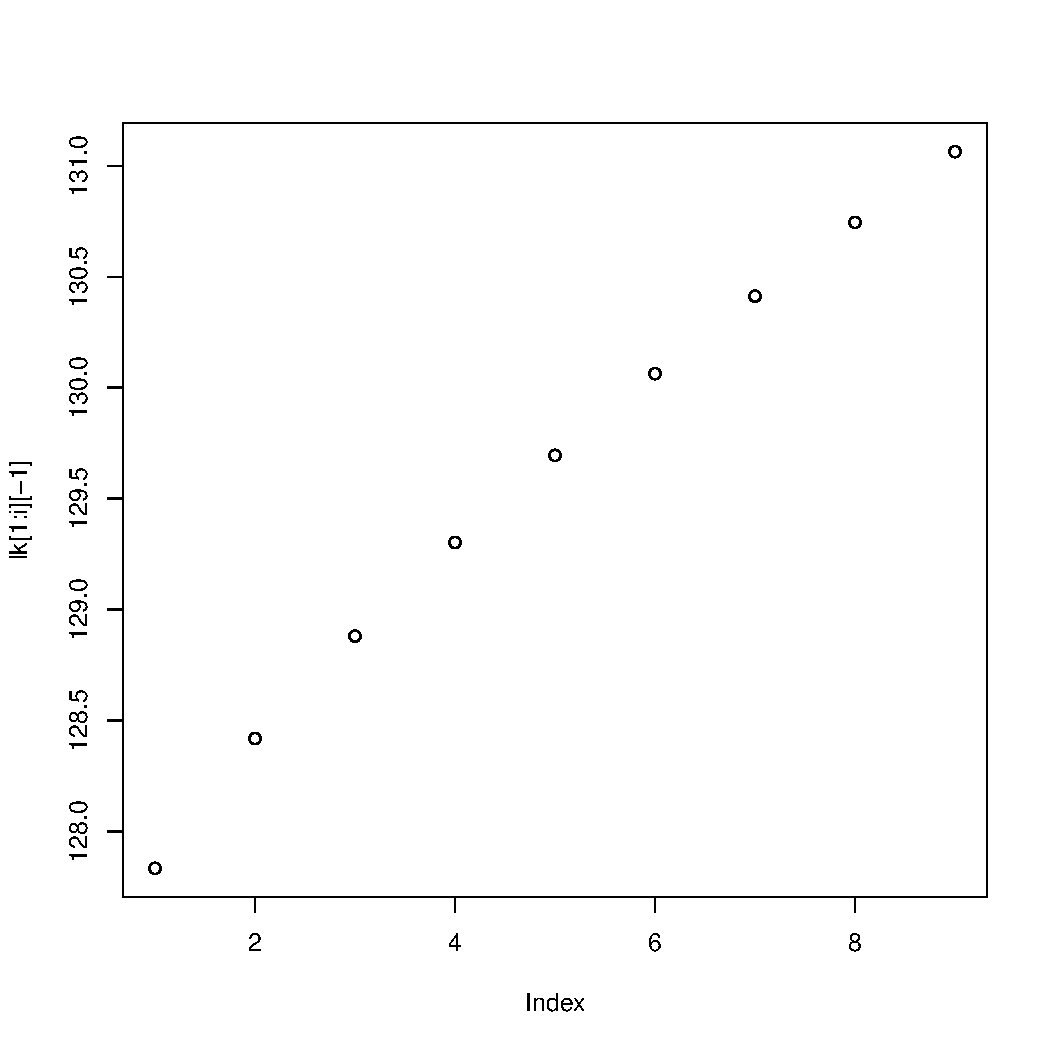
\includegraphics[width=\maxwidth]{figure/unnamed-chunk-1-1} 
\begin{kframe}\begin{alltt}
    \hlcom{## Point predict}
    \hlstd{HexPols_df} \hlkwb{<-} \hlkwd{SRE.predict}\hlstd{(S,}\hlkwc{use_centroid} \hlstd{= T)}

    \hlstd{X} \hlkwb{<-} \hlkwd{SpatialPolygons_to_df}\hlstd{(}\hlkwc{sp_polys} \hlstd{= HexPols_df,}
                               \hlkwc{vars} \hlstd{=} \hlkwd{c}\hlstd{(}\hlstr{"mu"}\hlstd{,}\hlstr{"var"}\hlstd{))}
\end{alltt}


{\ttfamily\noindent\itshape\color{messagecolor}{\#\# Joining by: "{}id"{}}}\begin{alltt}
    \hlstd{g1} \hlkwb{<-} \hlkwd{EmptyTheme}\hlstd{()} \hlopt{+}
        \hlkwd{geom_polygon}\hlstd{(}\hlkwc{data}\hlstd{=X,}\hlkwd{aes}\hlstd{(x,y,}\hlkwc{fill}\hlstd{=mu,}\hlkwc{group}\hlstd{=id),}
                     \hlkwc{colour}\hlstd{=}\hlstr{"light grey"}\hlstd{)} \hlopt{+}
        \hlkwd{scale_fill_distiller}\hlstd{(}\hlkwc{palette}\hlstd{=}\hlstr{"Spectral"}\hlstd{,}\hlkwc{trans}\hlstd{=}\hlstr{"reverse"}\hlstd{)} \hlopt{+}
        \hlkwd{geom_point}\hlstd{(}\hlkwc{data}\hlstd{=}\hlkwd{data.frame}\hlstd{(meuse),}
                   \hlkwd{aes}\hlstd{(x,y,}\hlkwc{fill}\hlstd{=}\hlkwd{log}\hlstd{(zinc)),}
                   \hlkwc{colour}\hlstd{=}\hlstr{"black"}\hlstd{,}
                   \hlkwc{pch}\hlstd{=}\hlnum{21}\hlstd{,} \hlkwc{size}\hlstd{=}\hlnum{3}\hlstd{)} \hlopt{+}
        \hlkwd{coord_fixed}\hlstd{()}

    \hlstd{g2} \hlkwb{<-} \hlkwd{EmptyTheme}\hlstd{()} \hlopt{+}
        \hlkwd{geom_polygon}\hlstd{(}\hlkwc{data}\hlstd{=X,}\hlkwd{aes}\hlstd{(x,y,}\hlkwc{fill}\hlstd{=}\hlkwd{sqrt}\hlstd{(var),}\hlkwc{group}\hlstd{=id),}
                     \hlkwc{colour}\hlstd{=}\hlstr{"light grey"}\hlstd{)} \hlopt{+}
        \hlkwd{scale_fill_distiller}\hlstd{(}\hlkwc{palette}\hlstd{=}\hlstr{"Spectral"}\hlstd{,}\hlkwc{trans}\hlstd{=}\hlstr{"reverse"}\hlstd{)} \hlopt{+}
        \hlkwd{geom_point}\hlstd{(}\hlkwc{data}\hlstd{=}\hlkwd{data.frame}\hlstd{(meuse),}
                   \hlkwd{aes}\hlstd{(x,y),}\hlkwc{colour}\hlstd{=}\hlstr{"black"}\hlstd{,}\hlkwc{pch}\hlstd{=}\hlnum{21}\hlstd{,} \hlkwc{size}\hlstd{=}\hlnum{3}\hlstd{)} \hlopt{+}
        \hlkwd{coord_fixed}\hlstd{()}

    \hlkwd{print}\hlstd{(g1)}
\end{alltt}
\end{kframe}
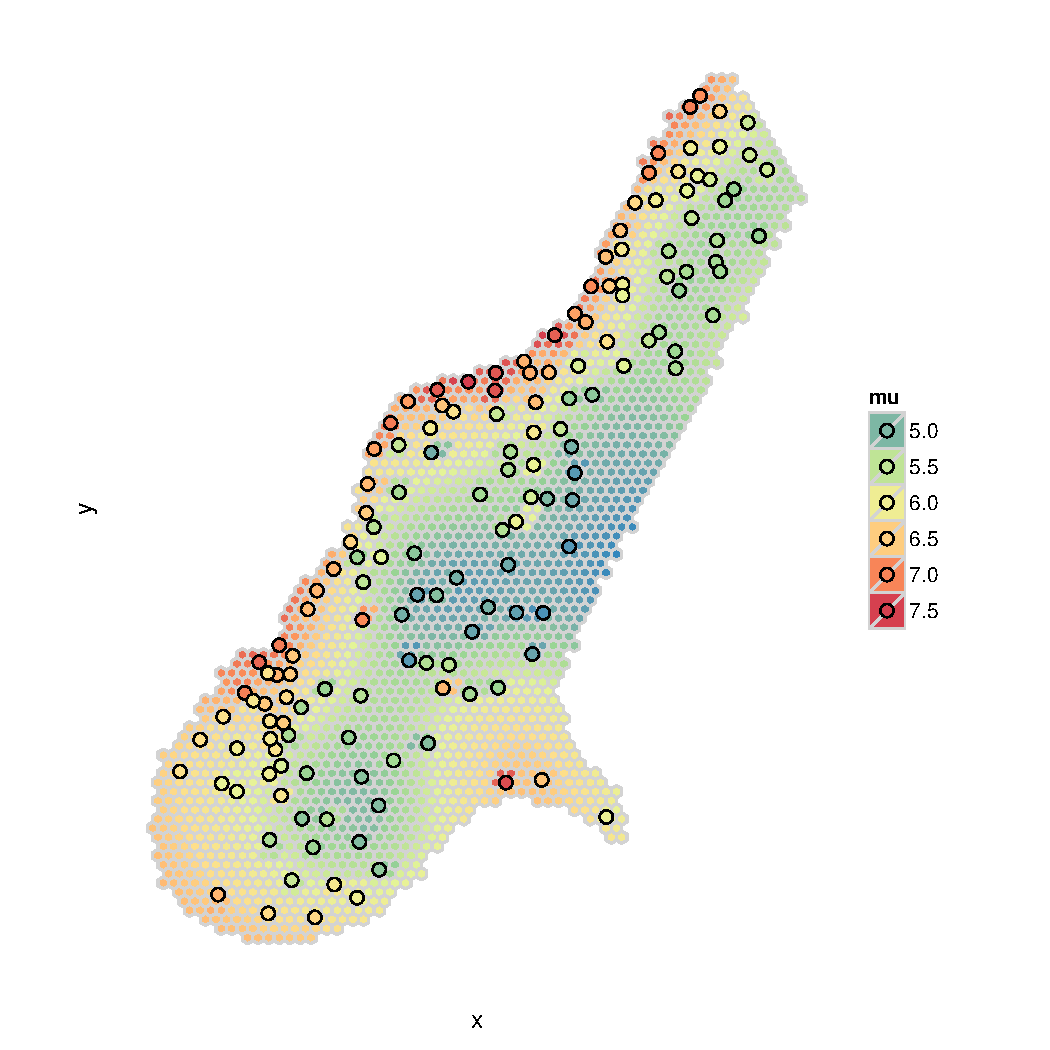
\includegraphics[width=\maxwidth]{figure/unnamed-chunk-1-2} 
\begin{kframe}\begin{alltt}
    \hlkwd{print}\hlstd{(g2)}
\end{alltt}
\end{kframe}
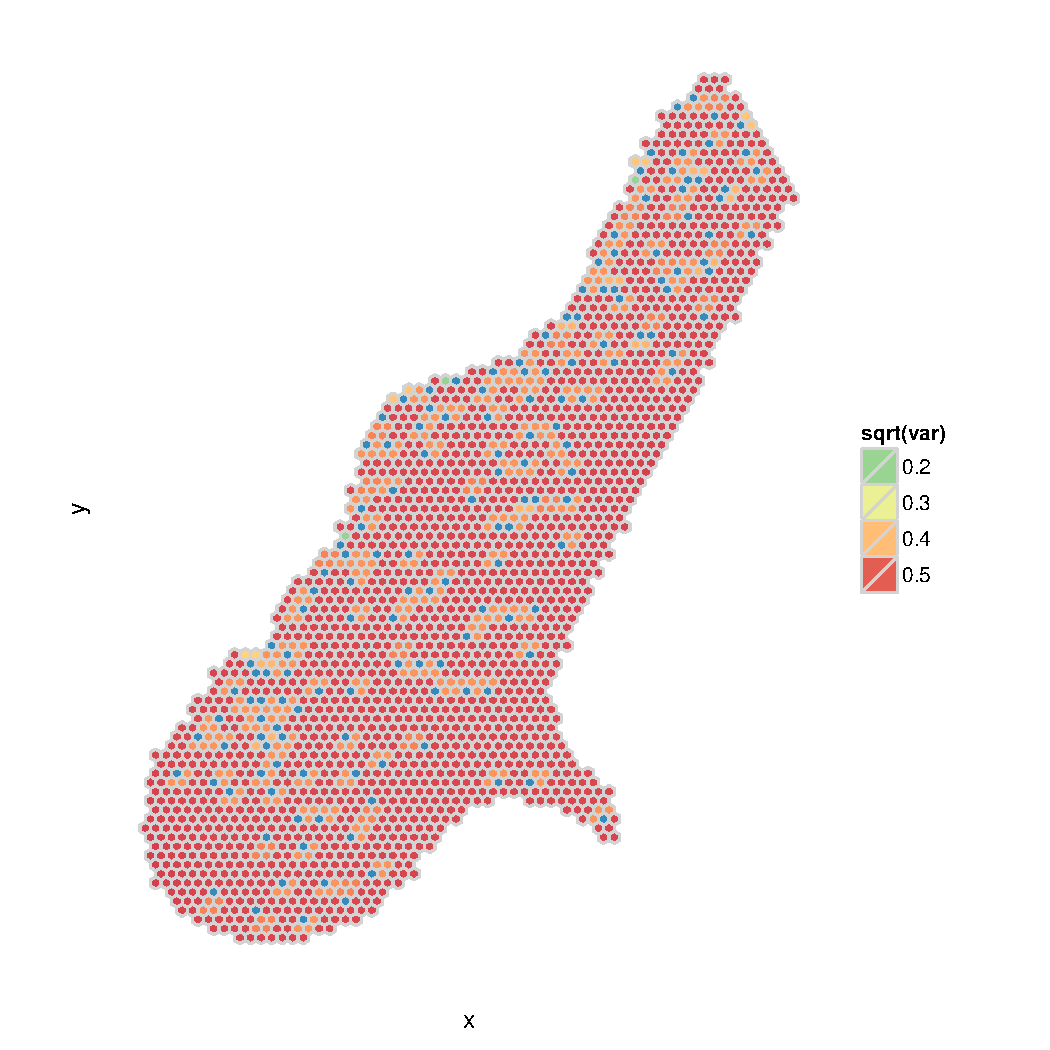
\includegraphics[width=\maxwidth]{figure/unnamed-chunk-1-3} 

\end{knitrout}

\begin{knitrout}
\definecolor{shadecolor}{rgb}{0.969, 0.969, 0.969}\color{fgcolor}\begin{kframe}
\begin{alltt}
\hlcom{## Load data}
\hlkwd{load}\hlstd{(}\hlkwd{system.file}\hlstd{(}\hlstr{"extdata"}\hlstd{,}\hlstr{"AIRS_05_2003.rda"}\hlstd{,} \hlkwc{package} \hlstd{=} \hlstr{"FRK"}\hlstd{))}
\hlstd{AIRS_05_2003} \hlkwb{<-} \hlkwd{filter}\hlstd{(AIRS_05_2003,day} \hlopt \hlnum{1}\hlstd{)} \hlopt
\hlkwd{select}\hlstd{(lon,lat,co2avgret)}
\hlkwd{coordinates}\hlstd{(AIRS_05_2003)} \hlkwb{=} \hlopt{~}\hlstd{lon}\hlopt{+}\hlstd{lat} \hlcom{# change into an sp object}
\hlkwd{proj4string}\hlstd{(AIRS_05_2003)}\hlkwb{=}\hlkwd{CRS}\hlstd{(}\hlstr{"+proj=longlat"}\hlstd{)}

\hlcom{## Prediction (BAU) grid}
\hlkwd{load}\hlstd{(}\hlkwd{system.file}\hlstd{(}\hlstr{"extdata"}\hlstd{,}\hlstr{"isea3h.rda"}\hlstd{,} \hlkwc{package} \hlstd{=} \hlstr{"FRK"}\hlstd{))}
\hlstd{isea3h_res} \hlkwb{<-} \hlkwd{filter}\hlstd{(isea3h,res} \hlopt{==} \hlnum{6}\hlstd{)} \hlopt
\hlkwd{arrange}\hlstd{(id)} \hlopt
\hlkwd{group_by}\hlstd{(id)} \hlopt
\hlkwd{filter}\hlstd{(}\hlkwd{diff}\hlstd{(}\hlkwd{range}\hlstd{(lon))} \hlopt{<} \hlnum{90}\hlstd{)} \hlopt
\hlkwd{data.frame}\hlstd{()} \hlopt
\hlkwd{mutate}\hlstd{(}\hlkwc{fs}\hlstd{=}\hlnum{1}\hlstd{)}

\hlstd{isea3h_sp_pol} \hlkwb{<-} \hlkwd{df_to_SpatialPolygons}\hlstd{(}
    \hlkwc{df}\hlstd{=}\hlkwd{filter}\hlstd{(isea3h_res,centroid}\hlopt{==}\hlnum{0}\hlstd{),}
    \hlkwc{keys}\hlstd{=}\hlkwd{c}\hlstd{(}\hlstr{"id"}\hlstd{),}
    \hlkwc{coords}\hlstd{=}\hlkwd{c}\hlstd{(}\hlstr{"lon"}\hlstd{,}\hlstr{"lat"}\hlstd{),}
    \hlkwc{proj}\hlstd{=}\hlkwd{CRS}\hlstd{(}\hlstr{"+proj=longlat"}\hlstd{))}

\hlstd{isea3h_sp_poldf} \hlkwb{<-} \hlkwd{SpatialPolygonsDataFrame}\hlstd{(}
    \hlstd{isea3h_sp_pol,}
    \hlkwd{cbind}\hlstd{(}\hlkwd{data.frame}\hlstd{(}\hlkwc{row.names}\hlstd{=}\hlkwd{names}\hlstd{(isea3h_sp_pol)),}
          \hlstd{(}\hlkwd{filter}\hlstd{(isea3h_res,centroid}\hlopt{==}\hlnum{1}\hlstd{)} \hlopt
               \hlkwd{select}\hlstd{(id,lon,lat,fs))))}

\hlcom{## Set up SRE model}
\hlstd{G} \hlkwb{<-} \hlkwd{auto_basis}\hlstd{(}\hlkwc{m} \hlstd{=} \hlkwd{sphere}\hlstd{(),}\hlkwc{data}\hlstd{=AIRS_05_2003,}
                \hlkwc{nres} \hlstd{=} \hlnum{3}\hlstd{,}\hlkwc{prune}\hlstd{=}\hlnum{15}\hlstd{,}\hlkwc{type} \hlstd{=} \hlstr{"bisquare"}\hlstd{)}
\end{alltt}
\begin{verbatim}
## [1] "Number of basis at resolution 1 = 32"
## [1] "Number of basis at resolution 2 = 90"
## [1] "Number of basis at resolution 3 = 258"
\end{verbatim}
\begin{alltt}
\hlstd{f} \hlkwb{<-} \hlstd{co2avgret} \hlopt{~} \hlstd{lat} \hlopt{+} \hlnum{1}
\hlstd{S} \hlkwb{<-} \hlkwd{SRE}\hlstd{(f,}\hlkwd{list}\hlstd{(AIRS_05_2003),G,isea3h_sp_poldf)} \hlopt
\hlkwd{SRE.fit}\hlstd{(}\hlkwc{n_EM} \hlstd{=} \hlnum{3}\hlstd{,}\hlkwc{print_lik}\hlstd{=T)}
\end{alltt}


{\ttfamily\noindent\color{warningcolor}{\#\# Warning in map\_data\_to\_BAUs(data[[i]], BAUs, av\_var = av\_var, variogram.formula = f): Not accounting for multiple data in the same grid box during variogram estimation. Need to see how to do this with gstat}}\begin{verbatim}
## [1] "sigma2e estimate = 3.52279378129999"
## [1] "Maximum EM iterations reached"
\end{verbatim}
\end{kframe}
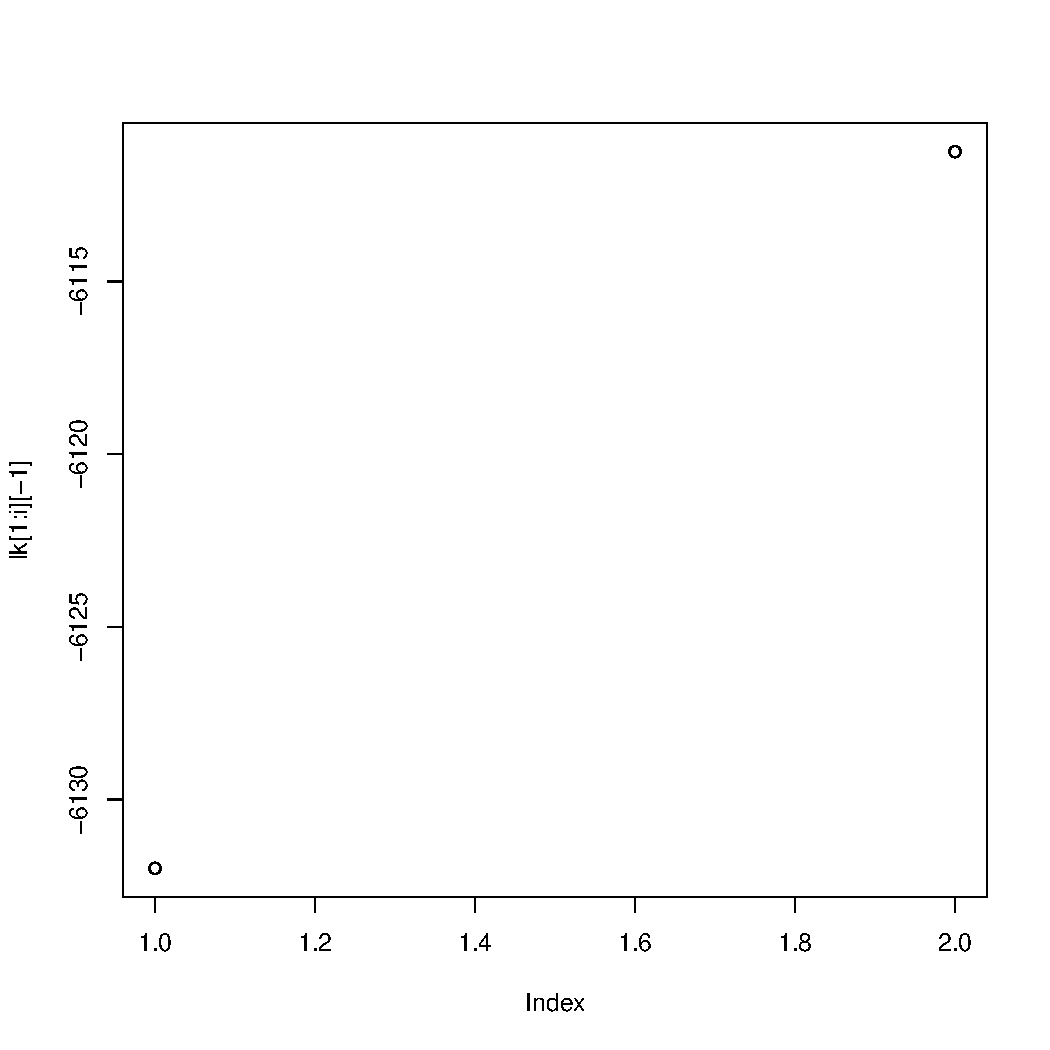
\includegraphics[width=\maxwidth]{figure/unnamed-chunk-2-1} 
\begin{kframe}\begin{alltt}
\hlstd{isea3h_sp_poldf} \hlkwb{<-} \hlkwd{SRE.predict}\hlstd{(S,}\hlkwc{use_centroid} \hlstd{= T)}

\hlstd{X} \hlkwb{<-} \hlkwd{SpatialPolygons_to_df}\hlstd{(}\hlkwc{sp_polys} \hlstd{= isea3h_sp_poldf,}
                           \hlkwc{vars} \hlstd{=} \hlkwd{c}\hlstd{(}\hlstr{"mu"}\hlstd{,}\hlstr{"var"}\hlstd{))}
\end{alltt}


{\ttfamily\noindent\itshape\color{messagecolor}{\#\# Joining by: "{}id"{}}}\begin{alltt}
\hlstd{g1} \hlkwb{<-} \hlstd{(}\hlkwd{EmptyTheme}\hlstd{()} \hlopt{+}
           \hlkwd{geom_polygon}\hlstd{(}\hlkwc{data}\hlstd{=X,}
                        \hlkwd{aes}\hlstd{(lon,lat,}\hlkwc{fill}\hlstd{=mu,}\hlkwc{group}\hlstd{=id),}
                        \hlkwc{colour}\hlstd{=}\hlstr{"light grey"}\hlstd{)} \hlopt{+}
           \hlkwd{scale_fill_distiller}\hlstd{(}\hlkwc{palette}\hlstd{=}\hlstr{"Spectral"}\hlstd{,}\hlkwc{trans}\hlstd{=}\hlstr{"reverse"}\hlstd{)} \hlopt{+}
           \hlkwd{coord_map}\hlstd{(}\hlstr{"mollweide"}\hlstd{))} \hlopt
\hlkwd{draw_world}\hlstd{(}\hlkwc{inc_border}\hlstd{=}\hlnum{FALSE}\hlstd{)}

\hlstd{mumin} \hlkwb{<-} \hlkwd{min}\hlstd{(X}\hlopt{$}\hlstd{mu)}
\hlstd{mumax} \hlkwb{<-} \hlkwd{max}\hlstd{(X}\hlopt{$}\hlstd{mu)}

\hlstd{g2} \hlkwb{<-} \hlstd{(}\hlkwd{EmptyTheme}\hlstd{()} \hlopt{+}
           \hlkwd{geom_point}\hlstd{(}\hlkwc{data}\hlstd{=}\hlkwd{data.frame}\hlstd{(AIRS_05_2003),}
                      \hlkwd{aes}\hlstd{(lon,lat,}
                          \hlkwc{colour}\hlstd{=}\hlkwd{pmin}\hlstd{(}\hlkwd{pmax}\hlstd{(}
                              \hlstd{co2avgret,mumin),}
                                      \hlstd{mumax)),}
                      \hlkwc{size}\hlstd{=}\hlnum{2}\hlstd{)} \hlopt{+}
           \hlkwd{scale_colour_distiller}\hlstd{(}\hlkwc{palette}\hlstd{=}\hlstr{"Spectral"}\hlstd{,}
                                  \hlkwc{trans}\hlstd{=}\hlstr{"reverse"}\hlstd{,}
                                  \hlkwd{guide_legend}\hlstd{(}\hlkwc{title}\hlstd{=}\hlstr{"co2"}\hlstd{)}
                                  \hlstd{)} \hlopt{+}
               \hlkwd{coord_map}\hlstd{(}\hlstr{"mollweide"}\hlstd{))} \hlopt
\hlkwd{draw_world}\hlstd{(}\hlkwc{inc_border}\hlstd{=}\hlnum{TRUE}\hlstd{)}

\hlkwd{print}\hlstd{(g1)}
\end{alltt}
\end{kframe}
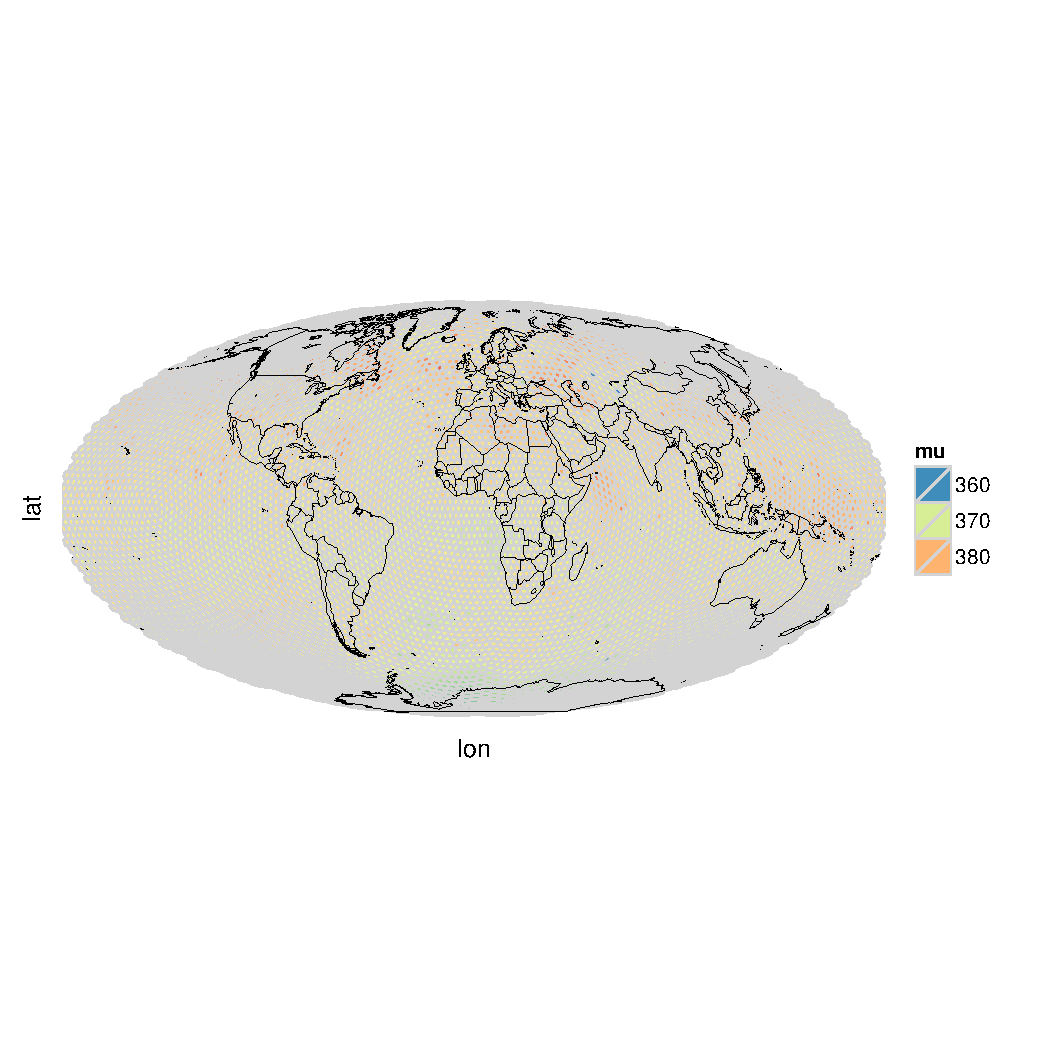
\includegraphics[width=\maxwidth]{figure/unnamed-chunk-2-2} 
\begin{kframe}\begin{alltt}
\hlkwd{print}\hlstd{(g2)}
\end{alltt}
\end{kframe}
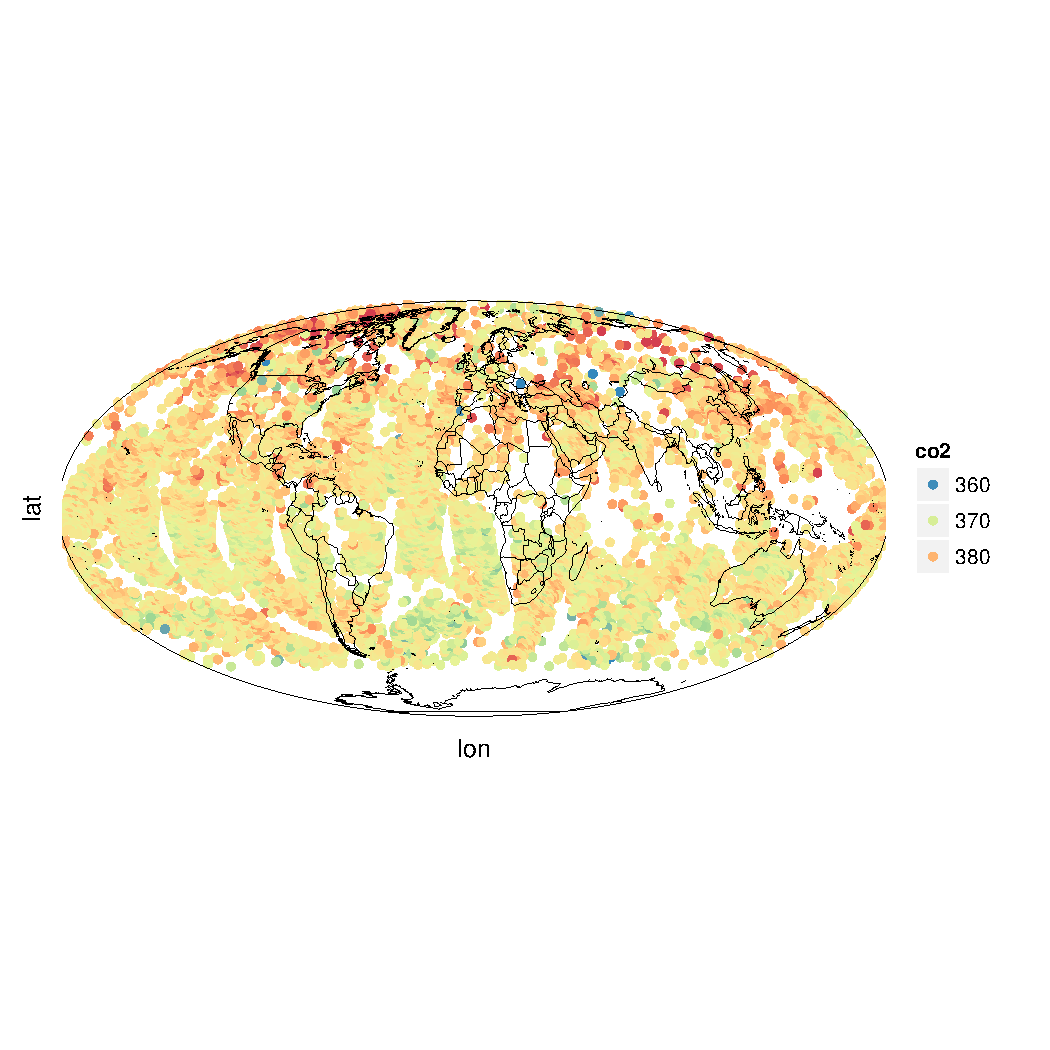
\includegraphics[width=\maxwidth]{figure/unnamed-chunk-2-3} 

\end{knitrout}


\end{document}
